\documentclass{article}

\usepackage{amsfonts}
\usepackage{mathtools}
\usepackage[a4paper, total={7.5in, 10.5in}]{geometry}
\usepackage{tikz}
\usetikzlibrary{automata, positioning}
\usetikzlibrary{arrows,backgrounds,snakes}

\title{Multimedia Grundlagen II - Zusammenfassung}

\newcommand{\prob}{\textit{P}}
\DeclareRobustCommand*{\tautequiv}{%
  \Relbar\joinrel\mathrel{|}
  \mathrel{|}\joinrel\Relbar%
}

\begin{document}
			\section*{Multimodale Analyse}
				\subsection*{Signale}
					\begin{align*}
						\textbf{Abtastsignal } & \text{Werte eines abgetasteten analogen Signals zu bestimmten Zeitpunkten}\\
						\textbf{Quantisierung } & \text{Bin\"are Repr\"asentation aller Abtastwerte}\\
						\textbf{Digitales Signal } & \text{Quantisiertes Abtastsignal}\\
						\textbf{Nyquist-Frequenz } & f_a = 2 \cdot f_{max}\\
					\end{align*}
				\subsection*{Klassifikation}
					\begin{align*}
						\textbf{Boxplot } & 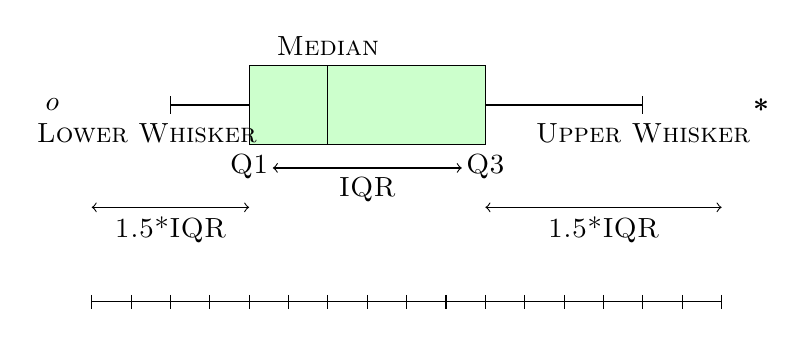
\begin{tikzpicture}
    \filldraw[fill=green!20] (2,0) rectangle (5,1);% draw the box
    \draw (3,0) -- (3,1) node[above]{$\textsc{Median}$};% draw the median
    \draw (5,0.5) -- (7,0.5);% draw right whisker
    \draw (2,0.5) -- (1,0.5);% draw left whisker
    \draw (7,0.39) -- (7,0.61) ;% draw vertical tab
    \draw (1,0.39) -- (1,0.61) ;% draw vertical tab
    \node[below] at (7, 0.39) {$\textsc{Upper Whisker}$};
    \node[below] at (0.7, 0.39) {$\textsc{Lower Whisker}$};
    \node[below] at (2,0) {$\textsc{Q1}$};% label the hinge
    \node[below] at (5,0) {$\textsc{Q3}$};% label the hinge
    \draw[<->] (2.3, -0.3) -- (4.7, -0.3)
        node[pos=0.5,below]{$\textsc{IQR}$}; % mark the IQR fences
    \draw[<->] (2, -0.8) -- (0,-0.8)
        node[pos=0.5,below]{$\textsc{1.5*IQR}$}; % left inner fence
    \draw[<->] (5, -0.8) -- (8,-0.8)
        node[midway,below]{$\textsc{1.5*IQR}$}; % right inner fence
    %
    \node[below] at (8.5,0.7) {$\textbf{*}$}; % mild outlier on the right
    \node[below] at (-0.5,0.7) {$o$}; % extreme outlier on the left
    % Axis
    \draw (0,-2) -- (8,-2);
    % Note that the snaked line is drawn to 11.1 to force
    % TikZ to draw the final tick.
    \draw[snake=ticks,segment length=0.5cm] (0,-2) -- (8,-2);
\end{tikzpicture}\\
						\textbf{Konfusionsmatrix } & x: \text{Klassenzugeh\"origkeit }, y: \text{Klassifikationsergebnis}\\
						\textbf{Overall accuracy } & \frac{\text{\#korrekt klassifizierte Instanzen}}{\text{\#alle Instanzen}}\\
						\textbf{Weighted accuracy } & \sum^{N}_{i=1} \frac{1}{N} \frac{\text{\#korrekt als Klasse $i$ klassifizierte Instanzen}}{\text{\#alle Instanzen in Klasse $i$}}\\
						\textbf{tp/tn/fp/fn } & \text{True/False Negatives/Positives}\\
						\textbf{Precision } & \frac{tp}{tp + fp}\\
						\textbf{Recall } & \frac{tp}{tp + fn}\\
						\textbf{M-Estimate } & \frac{n_{i,j} + m \cdot p}{n_j + m}\\
					\end{align*}
				\subsection*{Naive Bayes - Wahrscheinlichkeitstheorie}
					\begin{align*}
						D & \text{ Daten }\\
						h & \text{ Hypothese}\\
						\prob (h) & \text{ Warsch. dass $h$ erf\"ullt ist}\\
						\prob (D) & \text{ Warsch. dass $D$ beobachtet werden}\\
						\prob (D|h) & \text{ Warsch. dass mann $D$ beobachtet wenn $h$ erf\"ullt ist}\\
						\prob (h|D) & \text{ Warsch. dass $h$ bei $D$ gilt}\\
						h_{MAP} & \text{ argmax } \prob (h|D), h \in H\\
						h_{LM} & \text{ argmax } \prob (D|h), h \in H\\
					\end{align*}
				\subsection*{Hidden Markov Modelle}
					\begin{align*}
						\text{Modell } & \lambda\\
						\text{Zeitpunkt } & t\\
						\text{Zustand } & S_i, i = |S|\\
						\text{Beobachtung } & o_i, i = |o|\\
						\text{Zustandssequenz } & Q = q_1, q_2, \ldots, q_t\\
						\text{Beobachtungssequenz } & O = o_1, o_2, \ldots, o_t\\
						\end{align*}
						\begin{align*}
						\text{Forward Algorithmus } & t=1: \alpha_1(i) = \prob (o_1, o_2, \ldots, o_t, q_t = S_i|\lambda) & \text{Wahrscheinlichkeit da\ss}\\
						&\ \ \ \ \ \ \ \ \ \ \ \ \ \ \ \ \ \ \ \ \ = \pi_{S_i} * b_{S_i}(o_1), i = 1,\ldots, |S| & \text{O beobachtet wird}\\
						& t+1: \alpha_{t+1}(j) = \prob (o_1, o_2, \ldots, o_{t+1}, q_{t+1} = S_j|\lambda)\\
						&\ \ \ \ \ \ \ \ \ \ \ \ \ \ \ \ \ \ \ \ \ \ \ \ = \Bigg[\sum^{N}_{i=1} \alpha_{t}(i) a_{ij}\Bigg] b_j(o_{t+1})\\
						& 1 \leq t \leq T-1, 1 \leq j \leq N\\
						\text{Backward Algorithmus } & t=1: \beta_1(i) = \sum^{N}_{j=1}a_{ij}b_{j}(o_{t+1})\beta_{t+1}(j) & \text{Wahrscheinlichkeit da\ss}\\
						& 1 \leq t \leq T-1, 1 \leq i \leq N & \text{man sich in Zustand $S_i$ }\\
						& & \text{ befindet und beobachtet wird }\\
					\end{align*}
					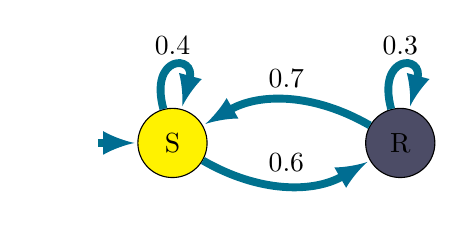
\begin{tikzpicture}
						% Add the states
						\node[state,
							  text=black,
							  draw=black,
							  fill=yellow] (s) {S};
						\node[state,
							  left=0.5cm of s,
							  text=white,
							  draw=white,
							  fill=white] (t) {};
						\node[state,
							  right=2cm of s,
							  text=black, 
							  draw=black,
							  fill={rgb:red,190;green,190;blue,255}] (r) {R};

						\draw[every loop,
						auto=right,
						line width=1mm,
						>=latex,
						draw={rgb:red,0;green,120;blue,150},
						fill={rgb:red,0;green,90;blue,120}]
							(s) edge[bend right, auto=left]  node {0.6} (r)
							(r) edge[bend right, auto=right] node {0.7} (s)
							(t) edge[auto=right] node {} (s)
							(s) edge[loop above]			 node {0.4} (s)
							(r) edge[loop above]			 node {0.3} (r);
							(2cm of s) edge[auto=left] node {0.5} (s)
					\end{tikzpicture}
					\hspace{-5.5cm}
					$\begin{bmatrix}
						A & 0.4\\
						B & 0.6\\
					\end{bmatrix}$
					\ \ \ \ \ \ \ \ \ \ \ \ \ \ \ \ \ \ \ \ \ \ \ \ \ \ \ \ \ \ \ \ \ \ \ \ \ \ \ \ \ \ \ \ \ \ $\begin{bmatrix}
						A & 0.3\\
						B & 0.7\\
					\end{bmatrix}$\\
					% \begin{tabular}{p{1cm}p{1cm}p{1cm}p{3cm}p{1cm}p{1cm}}
					% 	\text{Zeit } & t=1 & t=2 & t=3 & t=4 & t=5\\
					% 	\prob (S) & 1.0 & 0.4 & 0.4 * 0.4 + 0.6 * 0.7 & \\
					% 	\prob (R) &  & 0.6 & 0.6 + 0.6 * 0.3 & \\
					% 	\prob (A|S) & 0.4 &  & & \\
					% 	\prob (B|S) & 0.6 & 0.24 & & \\
					% 	\prob (A|R) &  & 0.18 & & \\
					% 	\prob (B|R) &  & 0.42 & & \\
					% \end{tabular}
	\subsection*{Neuronale Netze}
	\subsection*{Spracherkennung}
		\begin{align*}
			\textbf{Word Error Rate } & \frac{\text{Anzahl der fehlerhafte Worte}}{\text{Anzahl der Worte im korrekten Transkript}}\\
			\textbf{Ersetzungsfehler (S) } & \\
			\textbf{Auslassungsfehler (D) } & \\
			\textbf{Einf\"ugefehler (I) } & \\
			\textbf{Sprecherunabh\"angigkeit } & \text{Dialekte/Nicht-Muttersprachler/etc..}\\
			\textbf{Vokabular } & \text{Sorgf\"altige Kontrolle der Vokab.gr\"o\ss e/Behandlung von Worten, die sich nicht im Vokab. befinden}\\
			\textbf{Sprechweise } & \text{Isolierte Einzelw\"orter/mehrere Einzelw\"orter/flie\ss end gesprochene "normale" Sprache}\\
			\textbf{Umgebung } & \text{Hintergrundger\"ausche/Gespr\"ache (Crosstalk)}\\
			V\ & \text{Lexikongr\"o\ss e}\\
			N\ & \text{Anzahl der Worte im Text}\\
			\textbf{N-Gram } & \text{Unigram } \prob (w_i) = \frac{\text{count}(w_i)}{N} \xrightarrow{\text{adding-one}}{} \frac{\text{count}(w_i) + 1}{N + V}\\
			& \text{Bigram } \prob (w_i| w_{i-1}) = \frac{\text{count}(w_{n-1}w_{n})}{\text{count}(w_{n-1})} \xrightarrow{\text{adding-one}}{} \frac{\text{count}(w_{n-1}w_{n}) + 1}{\text{count}(w_{n-1}) + V}\\
			& \text{Trigram } \prob (w_i| w_{i-1}, w_{i-2})\\
			& \prob (w_i, w_{i+1}, w_{i+2}, w_{i+3}, w_{i+4}) = \prob (w_i | <start>) \prob (w_{i+1}|w_i) \prob (w_{i+2} | w_{i+1}) \prob (w_{i+3} | w_{i+2}) \prob (w_{i+4} | w_{i+3}) \prob (w_{i+5} | w_{i+4})\\
			\textbf{Perplexit\"at } & PP(w_1, \hdots, w_T) = \frac{1}{^T\sqrt{\prob (w_1, \hdots, w_T)}}\\
			\textbf{Absolute-discounting } & \\
		\end{align*}

\end{document}